In this section we analyse the effect of the adaptation module on the behaviour of the system. As already discussed in previous works (\cite{sandberg2002bayesian} for example), the role of adaptation is related with the presence of oscillations (sequential reactivation of the different patterns stored into the network). In the adopted model \cite{LansnerFRC} the adaptation acts as a local relaxation of the single minicolumns activity. 
 
 We will first focus on a system made by two hyper-columns each one made of 2 minicolumns interacting via their outputs.
 
 \paragraph{Assumptions}
 The assumptions presented below are kept fixed for the analysis that follows in this section:
 \begin{itemize}
     \item \textbf{A1} The matrix $W$ that describes the coupling of the units in the system is fixed, shaped by a previous learning experience.
     \item \textbf{A2} The coupling matrix is a diagonal matrix $W = \epsilon  I_{2}$ where $I_{2}$ is the 2-dimensional identity matrix. This choice corresponds to two stored orthogonal memory patterns. The parameter $\epsilon$ is a positive constant that parametrizes the coupling strength between the units. For simplicity in the notation the identity matrix will be written as $I$ without expliciting the dimension.
     \item \textbf{A3} The adaptation has a slower dynamics with respect to the activity dynamics of the minicolumns, therefore $\tau_a > 1$
 \end{itemize}
 
 \paragraph{System equations}
 Before going further with the analysis of the system with adaptation we recall the system's dynamics.
 
Denote $s_{11}, s_{12}, s_{21}, s_{22}$ the activities of the minicolumns grouped in the two hyper-columns $s_1 = [s_{11}, s_{12}]^T$ and $s_2 = [s_{21}, s_{22}]^T$;  $o_1 = [o_{11}, o_{12}]^T$ and $o_2 = [o_{21}, o_{22}]^T$ the corresponding outputs computed with the soft-max distribution; $W=\varepsilon I, \epsilon>0$ the interaction matrix between the two units. The interactions are symmetric in the sense that the coupling factor between unit $i$ and unit $j$ is equal to the coupling factor between unit $j$ and unit $i$.  The system dynamics follows:
\begin{equation}
\begin{aligned}
    \dot{s}_{11}&=-s_{11}-a_{11}+\varepsilon I o_{21} \\
    \tau_a \dot{a}_{11}&=g_a o_{11} - a_{11} \\
    \dot{s}_{12}&=-s_{12}-a_{12}+\varepsilon I o_{22} \\
    \tau_a \dot{a}_{12}&=g_a o_{12} - a_{12} \\
    \dot{s}_{21}&=-s_{21}-a_{21}+\varepsilon I o_{11} \\
    \tau_a \dot{a}_{21}&=g_a o_{21} - a_{21} \\
    \dot{s}_{22}&=-s_{22}-a_{22}+\varepsilon I o_{12} \\
    \tau_a \dot{a}_{22}&=g_a o_{22} - a_{22} \\
    o_{i j}&=\frac{e^{s_{i j}}}{\sum_{k=1}^{2} e^{s_{i k}}}
\end{aligned}
\label{eq:complete_dynamics}
\end{equation}
The system described in \eqref{eq:complete_dynamics} is a 8 dimensional system but its analysis can be easily simplified by exploiting some nice properties of the output softmax function. In particular the two following properties hold: 

\begin{equation}
 \sum_{k=1}^{N} o_{i k}=1
 \label{soft_sum}
\end{equation}
\begin{equation}
 f(d_i)= o_{i1}-o_{i2}=\frac{e^{d_i}-1}{e^{d_i}+1}, d_i = s_{i1}-s_{i2}
 \label{soft_diff}
\end{equation}

Given \eqref{soft_sum} and \eqref{soft_diff} we can introduce the following change of variables that will help us to significantly simplify the analysis of the dynamics and also get a deeper insight into the behaviour of our system. 

\begin{equation}
\begin{aligned}
z_i &= s_{i1} + s_{i2} \\
w_i &= a_{i1} + a_{i2} \\
d_i &= s_{i1} - s_{i2} \\
e_i &= a_{i1} - a_{i2} \\
\end{aligned}
\end{equation}
The dynamics in the new coordinate follows:

\begin{equation} 
\begin{aligned}
\dot z_i &= - z_i - w_i + \varepsilon, \forall i \in \{1,2\} \\
\tau_a \dot w_i &= g_a - w_i , \forall i \in \{1,2\} \\
\end{aligned}
\label{eq:diff_dynamics}
\end{equation}


\begin{equation} 
\begin{aligned}
\dot d_{1} &= - d_1 - e_1 + \varepsilon f(d_2) \\
\tau_a \dot{e}_{1} &= g_a f(d_1) - e_{1} \\
\dot d_{2} &= - d_2 - e_2 + \varepsilon f(d_1) \\
\tau_a \dot{e}_{2} &= g_a f(d_2) - e_{2} 
\end{aligned}
\label{eq:sum_dynamics}
\end{equation}


The dynamics of coupled variables $(z_i, w_i)$ is linear and it trivially holds that the equilibrium point $(z_i^*,w_i^*)=(-g_a+\varepsilon, g_a)$ is globally asymptotically stable. Furthermore, it is interesting to notice that the variables  $(z_i, w_i)$ are completely decoupled from $(d_i, e_i)$. The dynamics of the former it is much richer and requires further analysis. 
\paragraph{Synchronisation analysis}
One interesting property to be analysed is the synchronisation of the two units in \eqref{eq:sum_dynamics}. Therefore one could study the stability of the set $M = \{d_1, e_1, d_2, e_2 : d_1 = d_2,\ e_1 = e_2 \}$. From some preliminary experiments (\cref{fig:2_2_synch}), this hypothesis looks plausible, therefore it is worthwhile to try to prove this statement.

 \begin{figure}[!h]
        \center{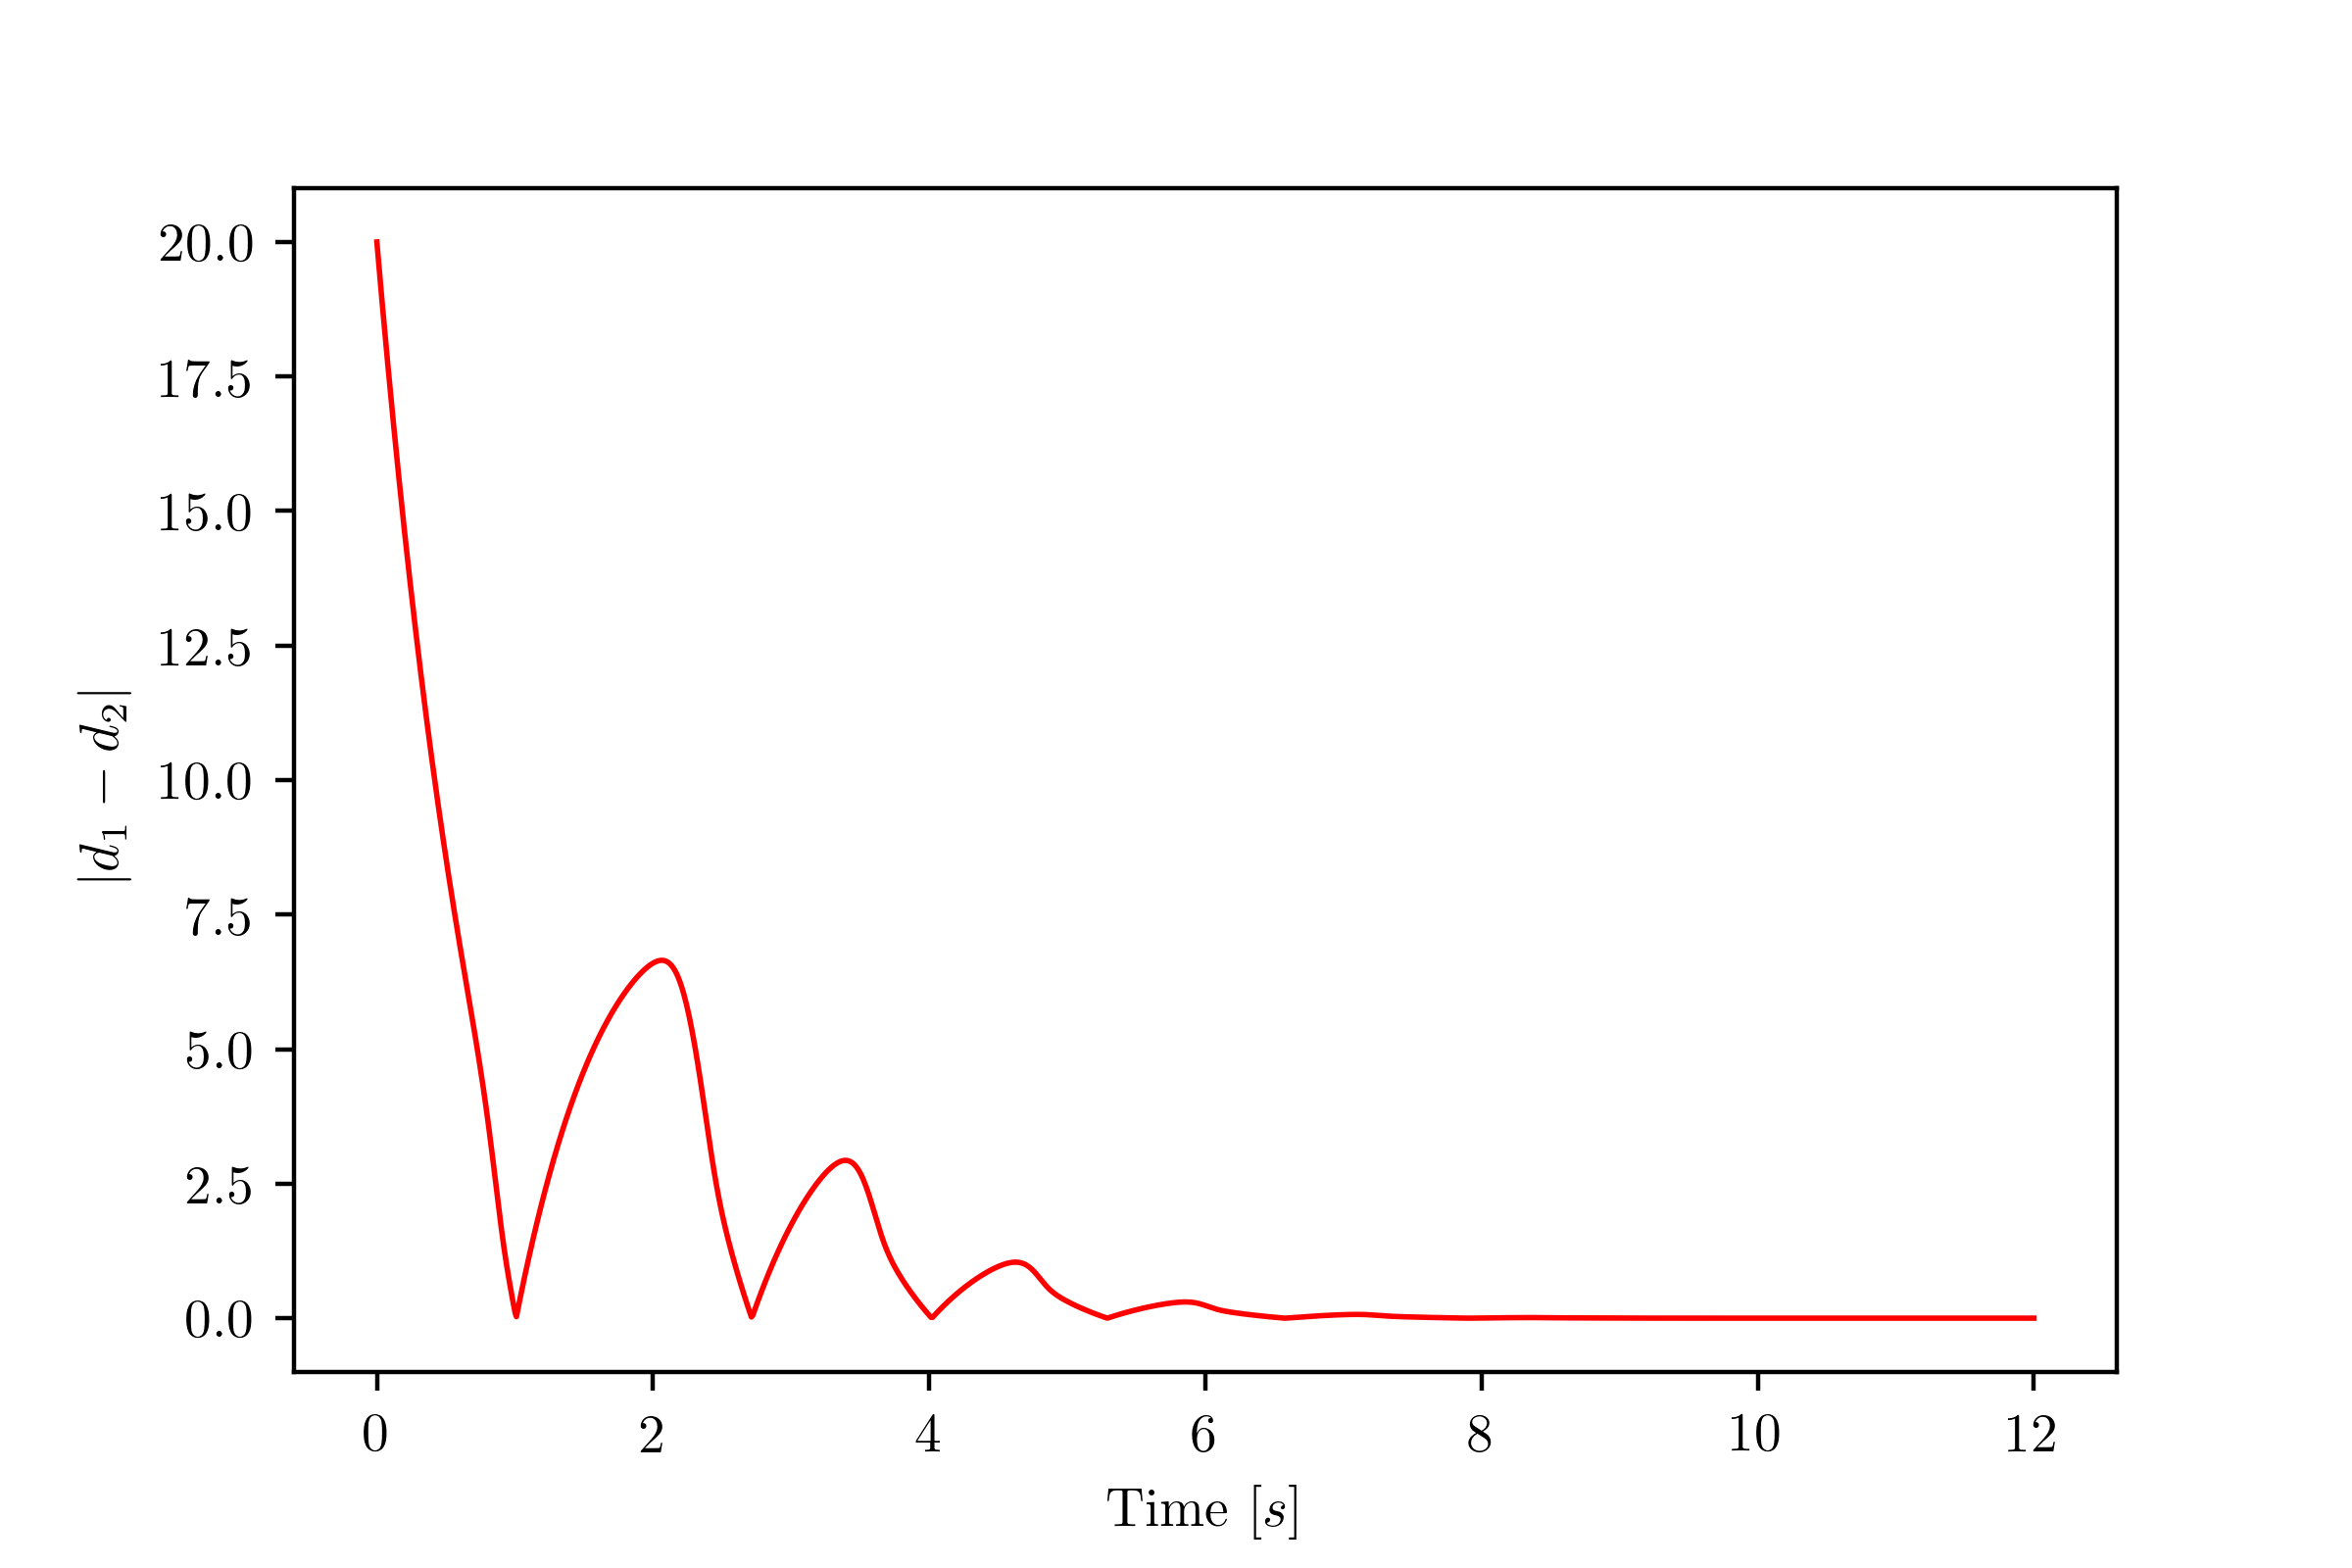
\includegraphics[width=\textwidth]{text/analysis/fig/2by2adapt/synch_2_by_2.png}}
        \caption{\label{fig:2_2_synch} Dynamics of the absolute error $|d_1-d_2|$}
\end{figure}

In order to study the stability of the synchronisation set $M$, one can study the error dynamics $d=d_1 - d_2$ and $e= e_1 - e_2$ and its stability. 

\begin{equation} 
\begin{aligned}
\dot d &= -d - e - \varepsilon \cdot (f(d_1) - f(d_2)) \\
\tau_e \dot e &= g_a \cdot (f(d_1) - f(d_2)) - e
\end{aligned}
\end{equation}


 We would like to replace the quantity $f(d_1) - f(d_2)$ with some function of the only difference of $d=d_1-d_2$. Unfortunately, this is not possible since $f(d_1)-f(d_2) = \frac{e^{d_1}-e^{d_2}}{(1+e^{d_1})(1+e^{d_2})}$. Nevertheless it could be interesting to see $f(d_1)-f(d_2)$ as a time-varying function $g(d, t)$ and analyse some properties that are preserved during the evolution of the system.
It is easy to prove that:
\begin{equation}
\begin{aligned}
|g(d,t)| &\leq \frac{1}{2}d(t) \\
g(d,t)&d>0, \forall t, d\neq0
\end{aligned}
\end{equation}
\textbf{Missing part about Lyapunov stability analysis.}

\paragraph{Bifurcation Analysis}
Once we have proven that the synchronisation manifold (or set) is Globally Asymptotically Stable we can study the dynamics of the system restricted on it. Remember that in $M$ it holds that $d_1=d_2$, therefore we can study the dynamics of the two identical units independently.  
\begin{equation}
\begin{aligned}
\dot d_{1} &= - d_1 - e_1 + \varepsilon f(d_1) \\
\tau_a \dot{e}_{1}&=g_a f(d_1) - e_{1}\\
f(d_1) &= \frac{e^{d_1}-1}{e^{d_1}+1}
\end{aligned}
\label{eq:2D_sync}
\end{equation}

We will start the analysis of this two dimensional system by computing the equilibria $(d_1^*,e_1^*)$ and study their properties with the variation of the parameters $\varepsilon, g_a$. The time constant $\tau_a$ is kept fixed, considered as a typical constant of the system. Notice that the system has a global symmetry property: for each solution $(d_1(t), e_1(t))$ it holds that also $(-d_1(t), -e_1(t))$ is a solution. The roots of the equations below \eqref{eq:eq_d_eq}, \eqref{eq:eq_e_eq}  are the fixed points of the dynamics in \eqref{eq:2D_sync}.
\begin{equation}
 (\varepsilon - g_a)f(d_1^*) - d_1^* = 0
\label{eq:eq_d_eq}
\end{equation}
\begin{equation}
e_1^* = g_a f(d_1^*)
\label{eq:eq_e_eq}
\end{equation}

The number of equilibria is uniquely defined by the quantity $\varepsilon-g_a$. In particular, it is easy to show analitically that there is a unique equilibrium for $\varepsilon \leq g_a-2$, while for $\varepsilon > g_a-2$ we have three equilibrium points. Unfortunately, since the equilibria can not be computed analytically we will make use of numerical analysis. In \cref{fig:eq2D_adapt} the three most important cases are plotted.

 \begin{figure}[!h]
        \center{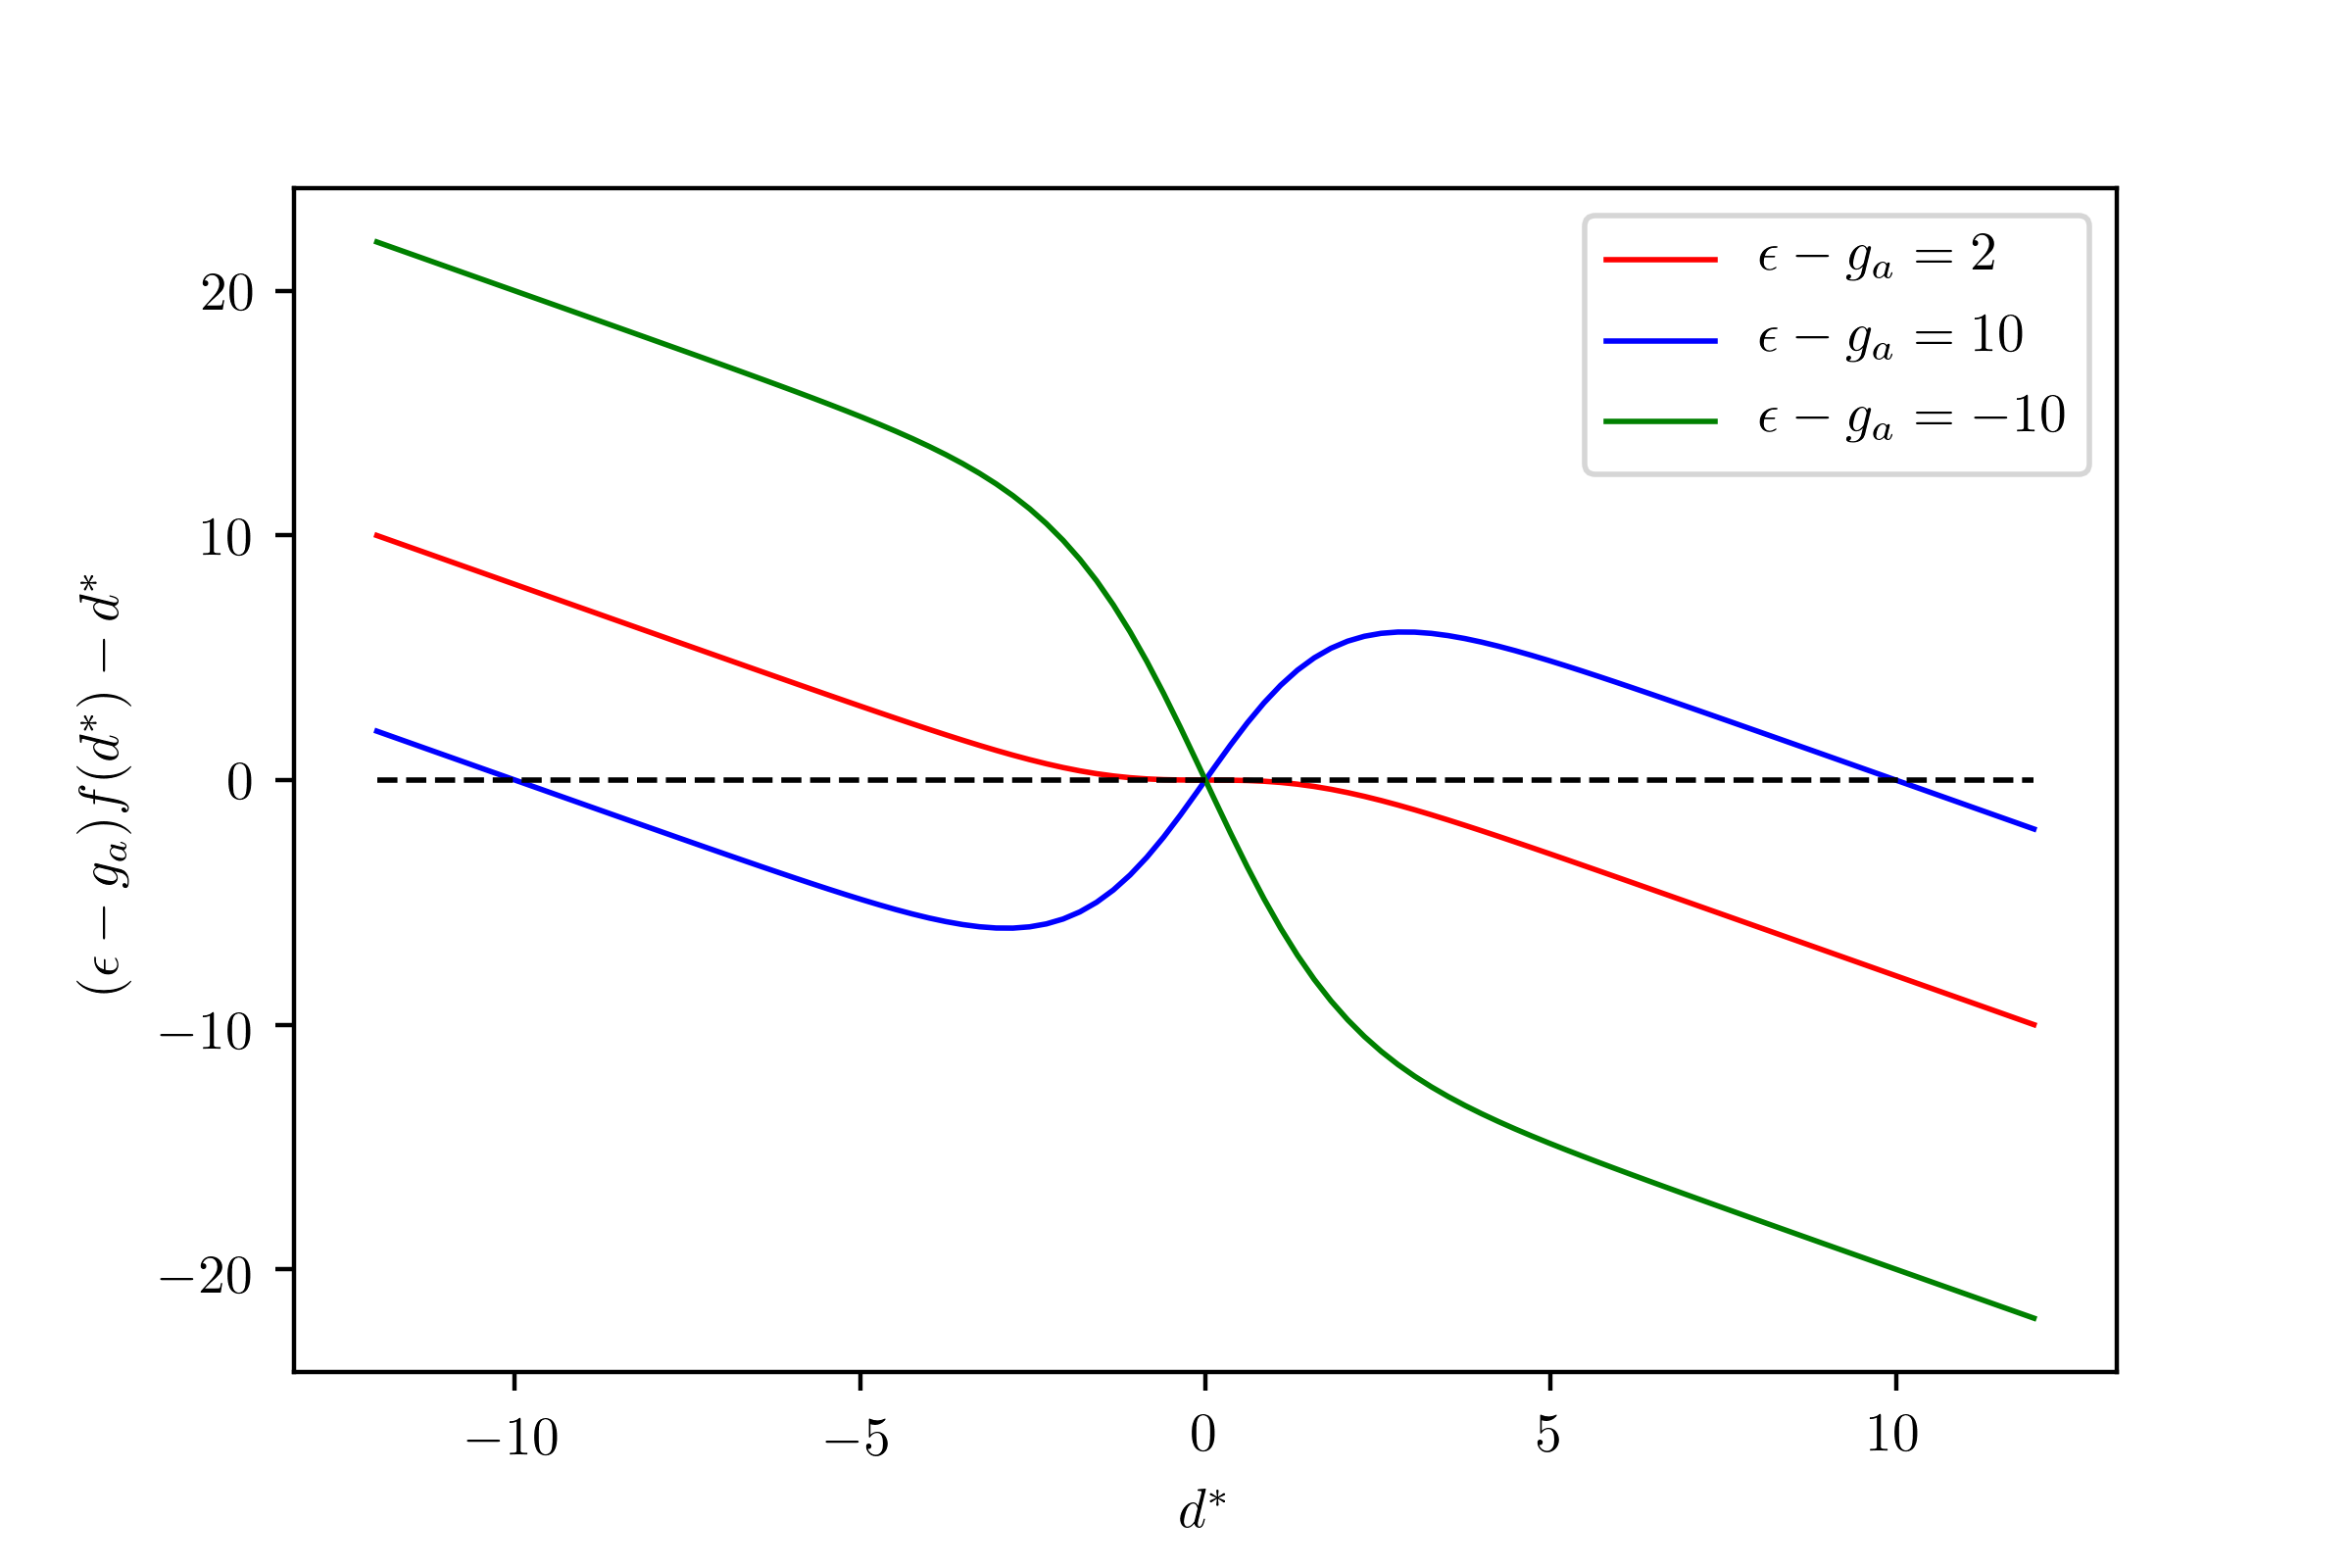
\includegraphics[width=\textwidth]{text/analysis/fig/2by2adapt/equilibria_2D.png}}
        \caption{\label{fig:eq2D_adapt} Graphical visualization of the roots of the equation in \eqref{eq:eq_d_eq}} with varying the quantity $\varepsilon - g_a$.
\end{figure}

We will first analyse the system with $\varepsilon - g_a < 2$. With this choice of parameters the unique equilibrium is the point $(d_1^*,e_1^*)=(0, 0)$. The computed jacobian matrix $J_{(0,0)}$ and the characteristic polynomial are the following:

\begin{equation}
J_{(0, 0)} = \begin{bmatrix} 
\frac{\varepsilon}{2} & -1 \\
\frac{g_a}{2\tau_a} & -\frac{1}{\tau}
\end{bmatrix}
\end{equation}

\begin{equation}
\rho(\lambda) = \lambda^2 +  \frac{2\tau_a + 2 - \tau_a \varepsilon}{2\tau_a} \lambda + \frac{-2\varepsilon + 2g_a + 4}{4\tau_a}
\end{equation}

\begin{equation}
\rho(\lambda) = \lambda^2 + a\lambda +b
\end{equation}

In order to study the stability of the equilibrium point one can study the sign of the polynomial's coefficient. In fact for a second order polynomial, the number of roots with positive real part can be determined by the number of variations in the polynomial's coefficients \cite{gantmacher2005matrix}.

\begin{equation}
\begin{aligned}
 a < 0 \iff & \varepsilon > 2(1 + \frac{1}{\tau_a}) \\
 b < 0 \iff & \varepsilon > g_a + 2
\end{aligned}
\end{equation}

When $\varepsilon<2(1+\frac{1}{\tau_a})$ the origin is an asymptotically stable equilibrium point. This condition is not particularly interesting since it means that all the units in the network converge to the same value and their output is identical. In other words, the network is not able to recall any pattern (\cref{fig:eq2D_focus}).

\begin{figure}[!h]
        \center{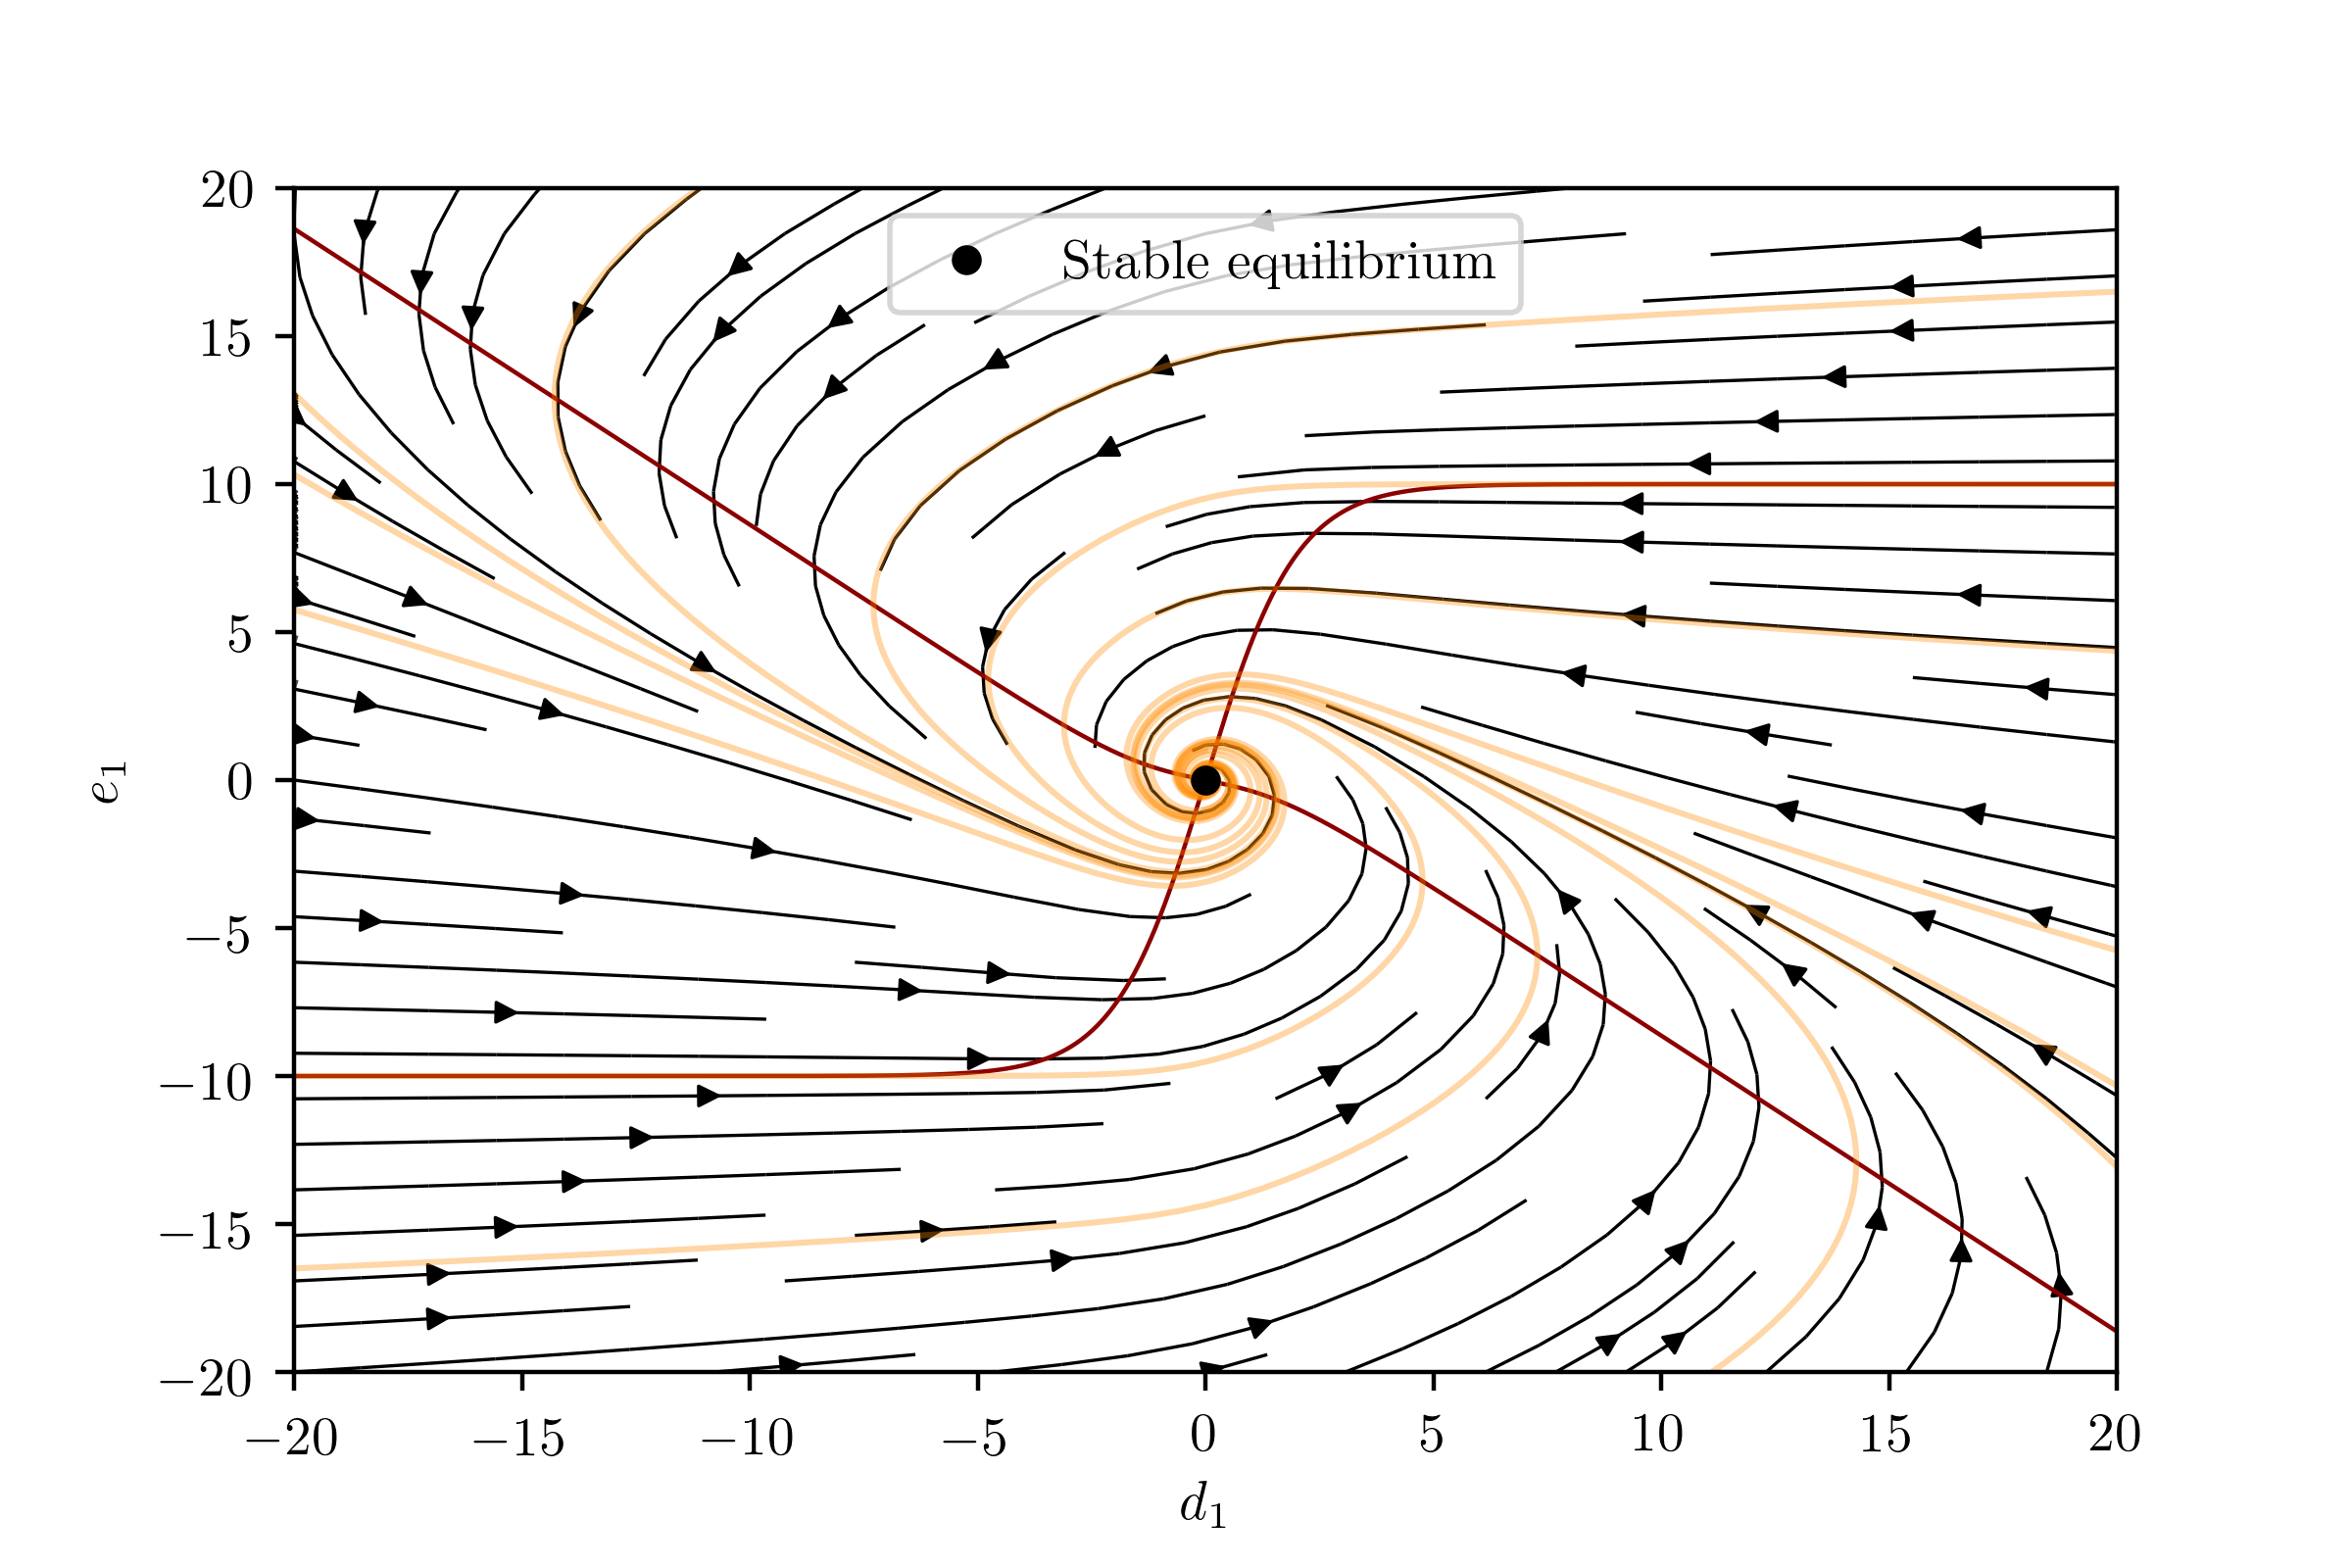
\includegraphics[width=\textwidth]{text/analysis/fig/2by2adapt/streamline_stable_focus.png}}
        \caption{\label{fig:eq2D_focus} Phase portrait of system in \eqref{eq:2D_sync} for $\varepsilon=1.5,\ g_a=10,\ \tau_a=2$. The nullclines are shown in dark red; the streamline plot is shown in black; several trajectories of the system with different initial conditions are shown in orange.}
\end{figure}


At the critical value $\varepsilon^* = 2 ( 1 + \frac{1}{\tau_a} ) $ a \textbf{supercritical Hopf} bifurcation occurs. In fact, as $\varepsilon$ passes through $\varepsilon^*$, the complex eigenvalues $\lambda_{1,2}$ crosses the imaginary axis. In fact, ${\rm I\!R}(\lambda_{1,2})<0, \varepsilon < \varepsilon^*$ and  ${\rm I\!R}(\lambda_{1,2})>0, \varepsilon > \varepsilon^*$. Therefore, the equilibrium point $(0, 0)$ changes its stability and a unique stable limit cycle bifurcates from it (\cref{fig:eq2D_cycle}).
\begin{figure}[!h]
        \center{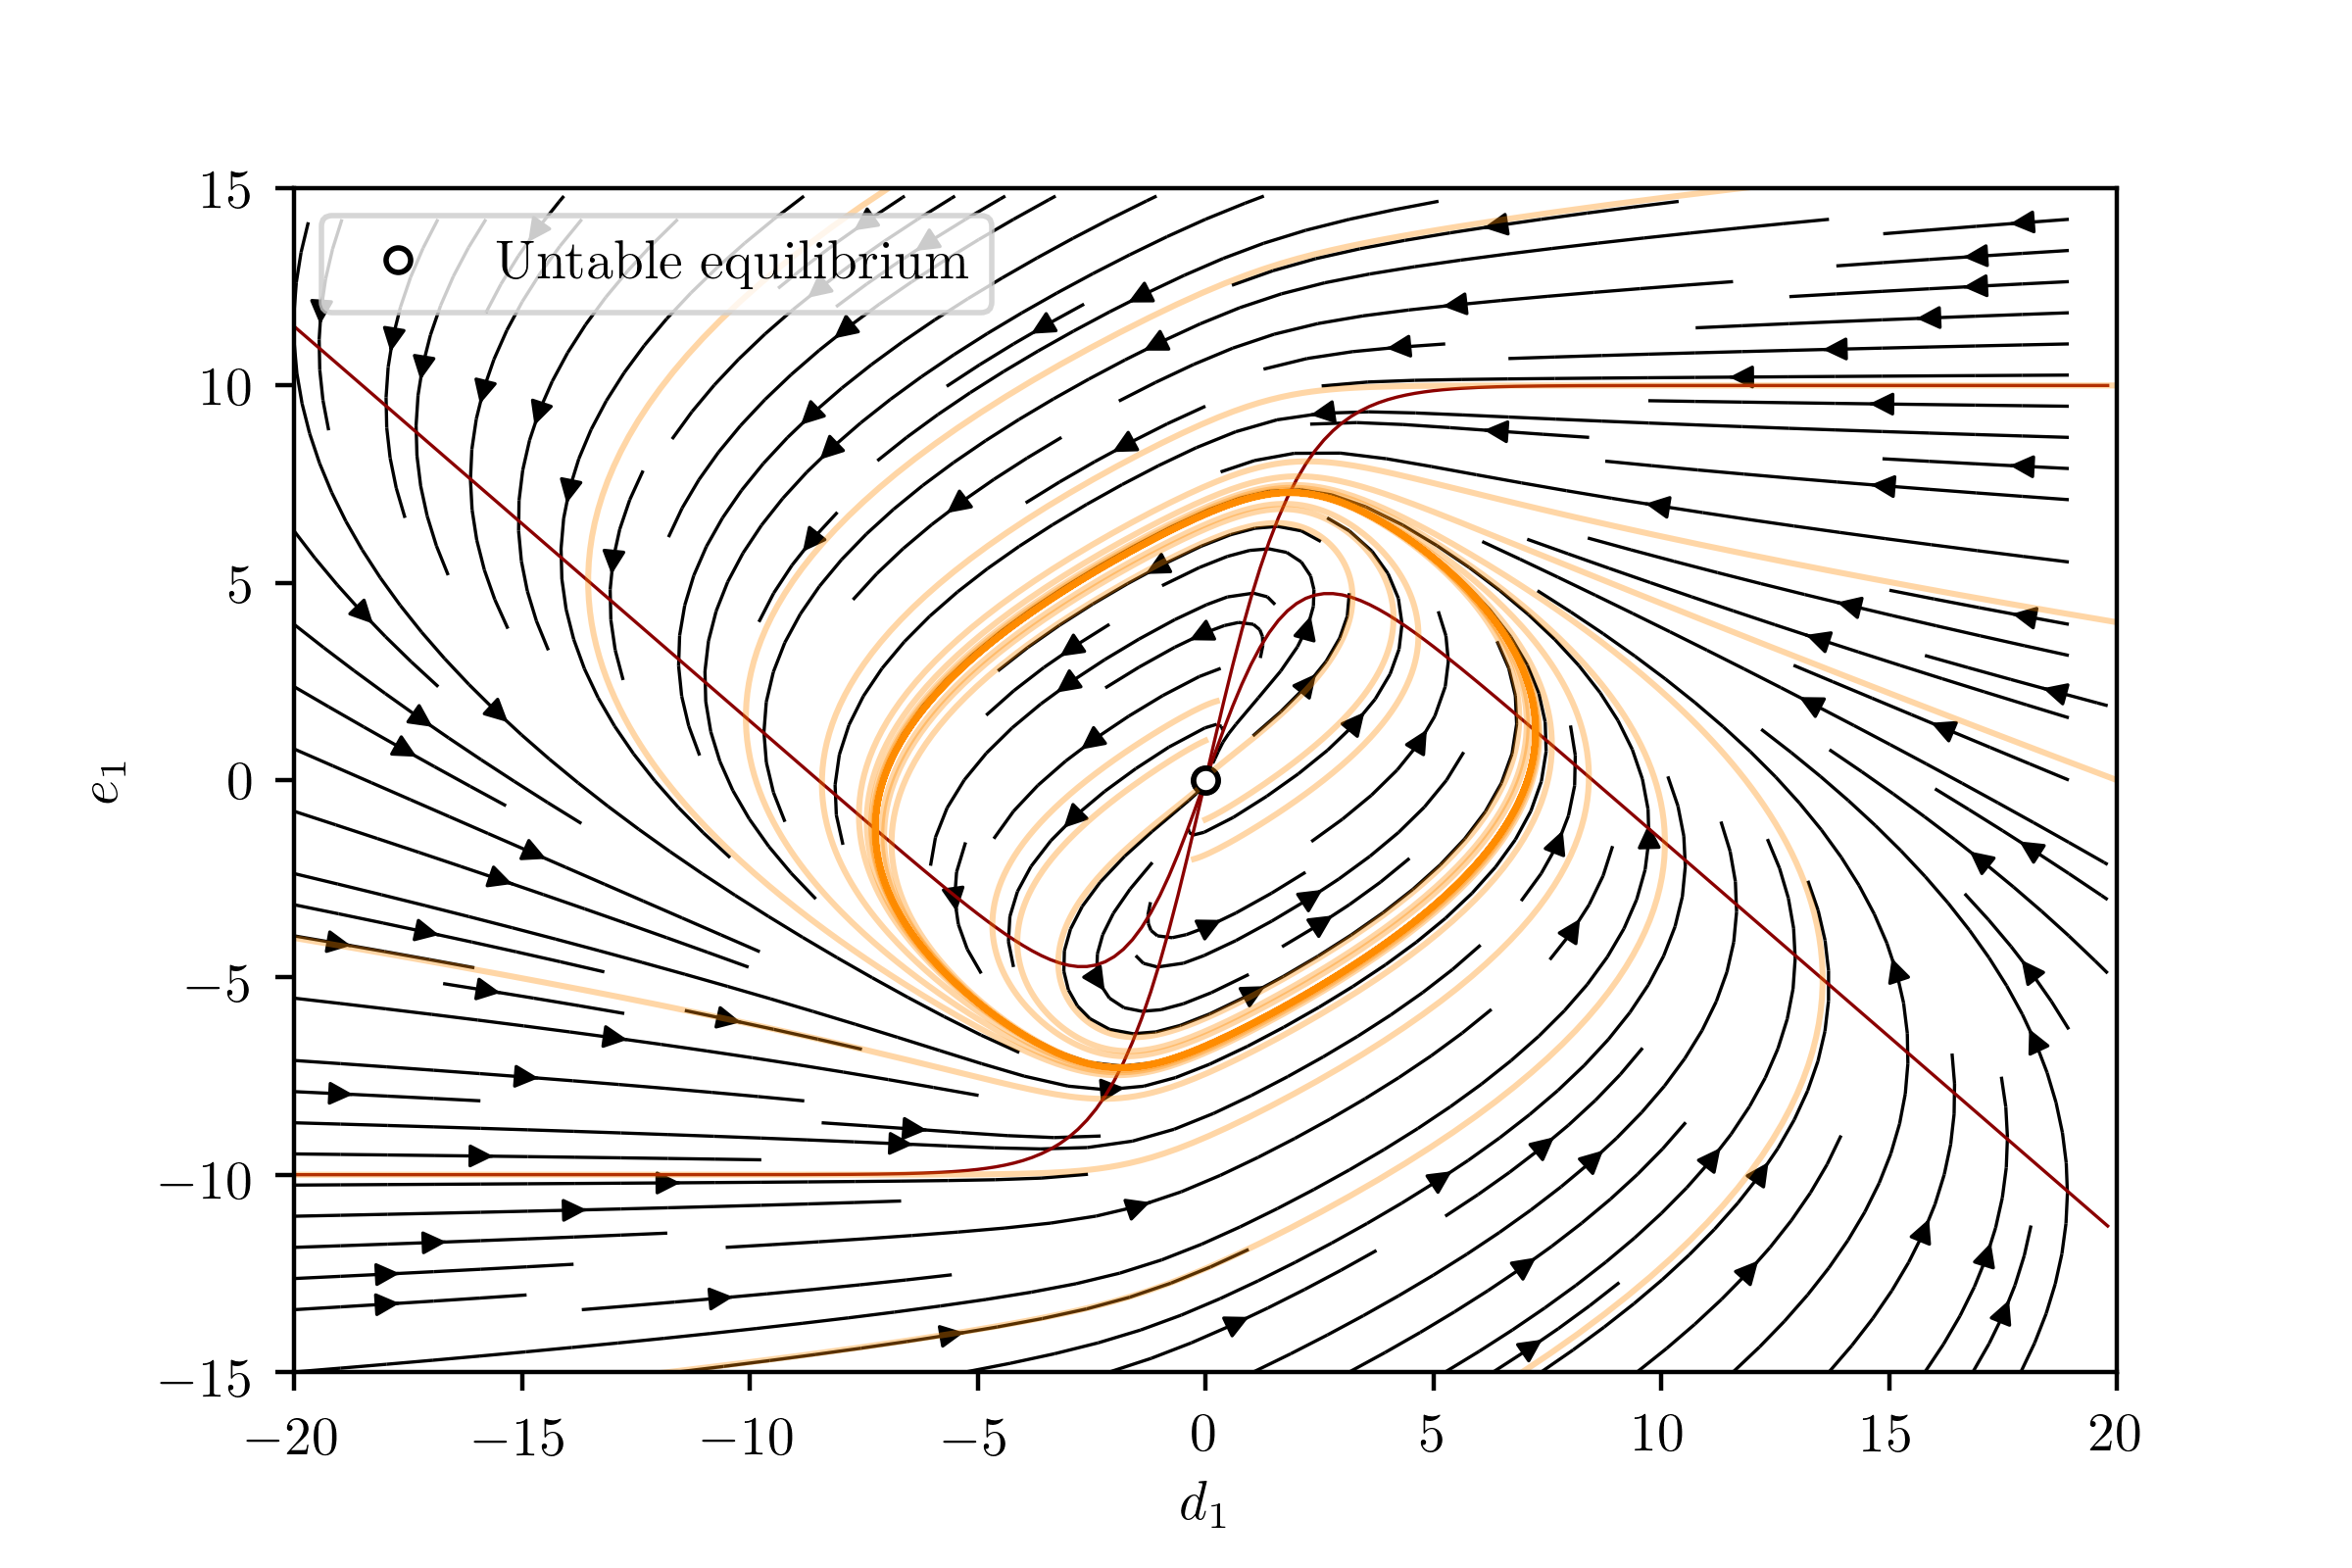
\includegraphics[width=\textwidth]{text/analysis/fig/2by2adapt/streamline_cycle.png}}
        \caption{\label{fig:eq2D_cycle} Phase portrait of system in \eqref{eq:2D_sync} for $\varepsilon=8.5,\ g_a=10,\ \tau_a=2$. The nullclines are shown in dark red; the streamline plot is shown in black; several trajectories of the system with different initial conditions are shown in orange.}
\end{figure}


But what happens when the coupling factor $\varepsilon$ increases? The next interesting bifurcation phenomenon occurs at the critical value $\varepsilon^o = g_a + 2$ when a \textbf{supercritical pitchfork bifurcation} occurs. In fact, the origin spawns two unstable equilibria and \textit{changes from unstable node to saddle node. What counts for bifurcations is what happens on the center manifold}. While the parameter $\epsilon > \epsilon^o$ keeps increasing the additional two equilibria moves far away from the origin and additional bifurcations occur. In particular, one can numerically find that at ... hopf bifurcation happens again.


\begin{figure}[!h]
        \center{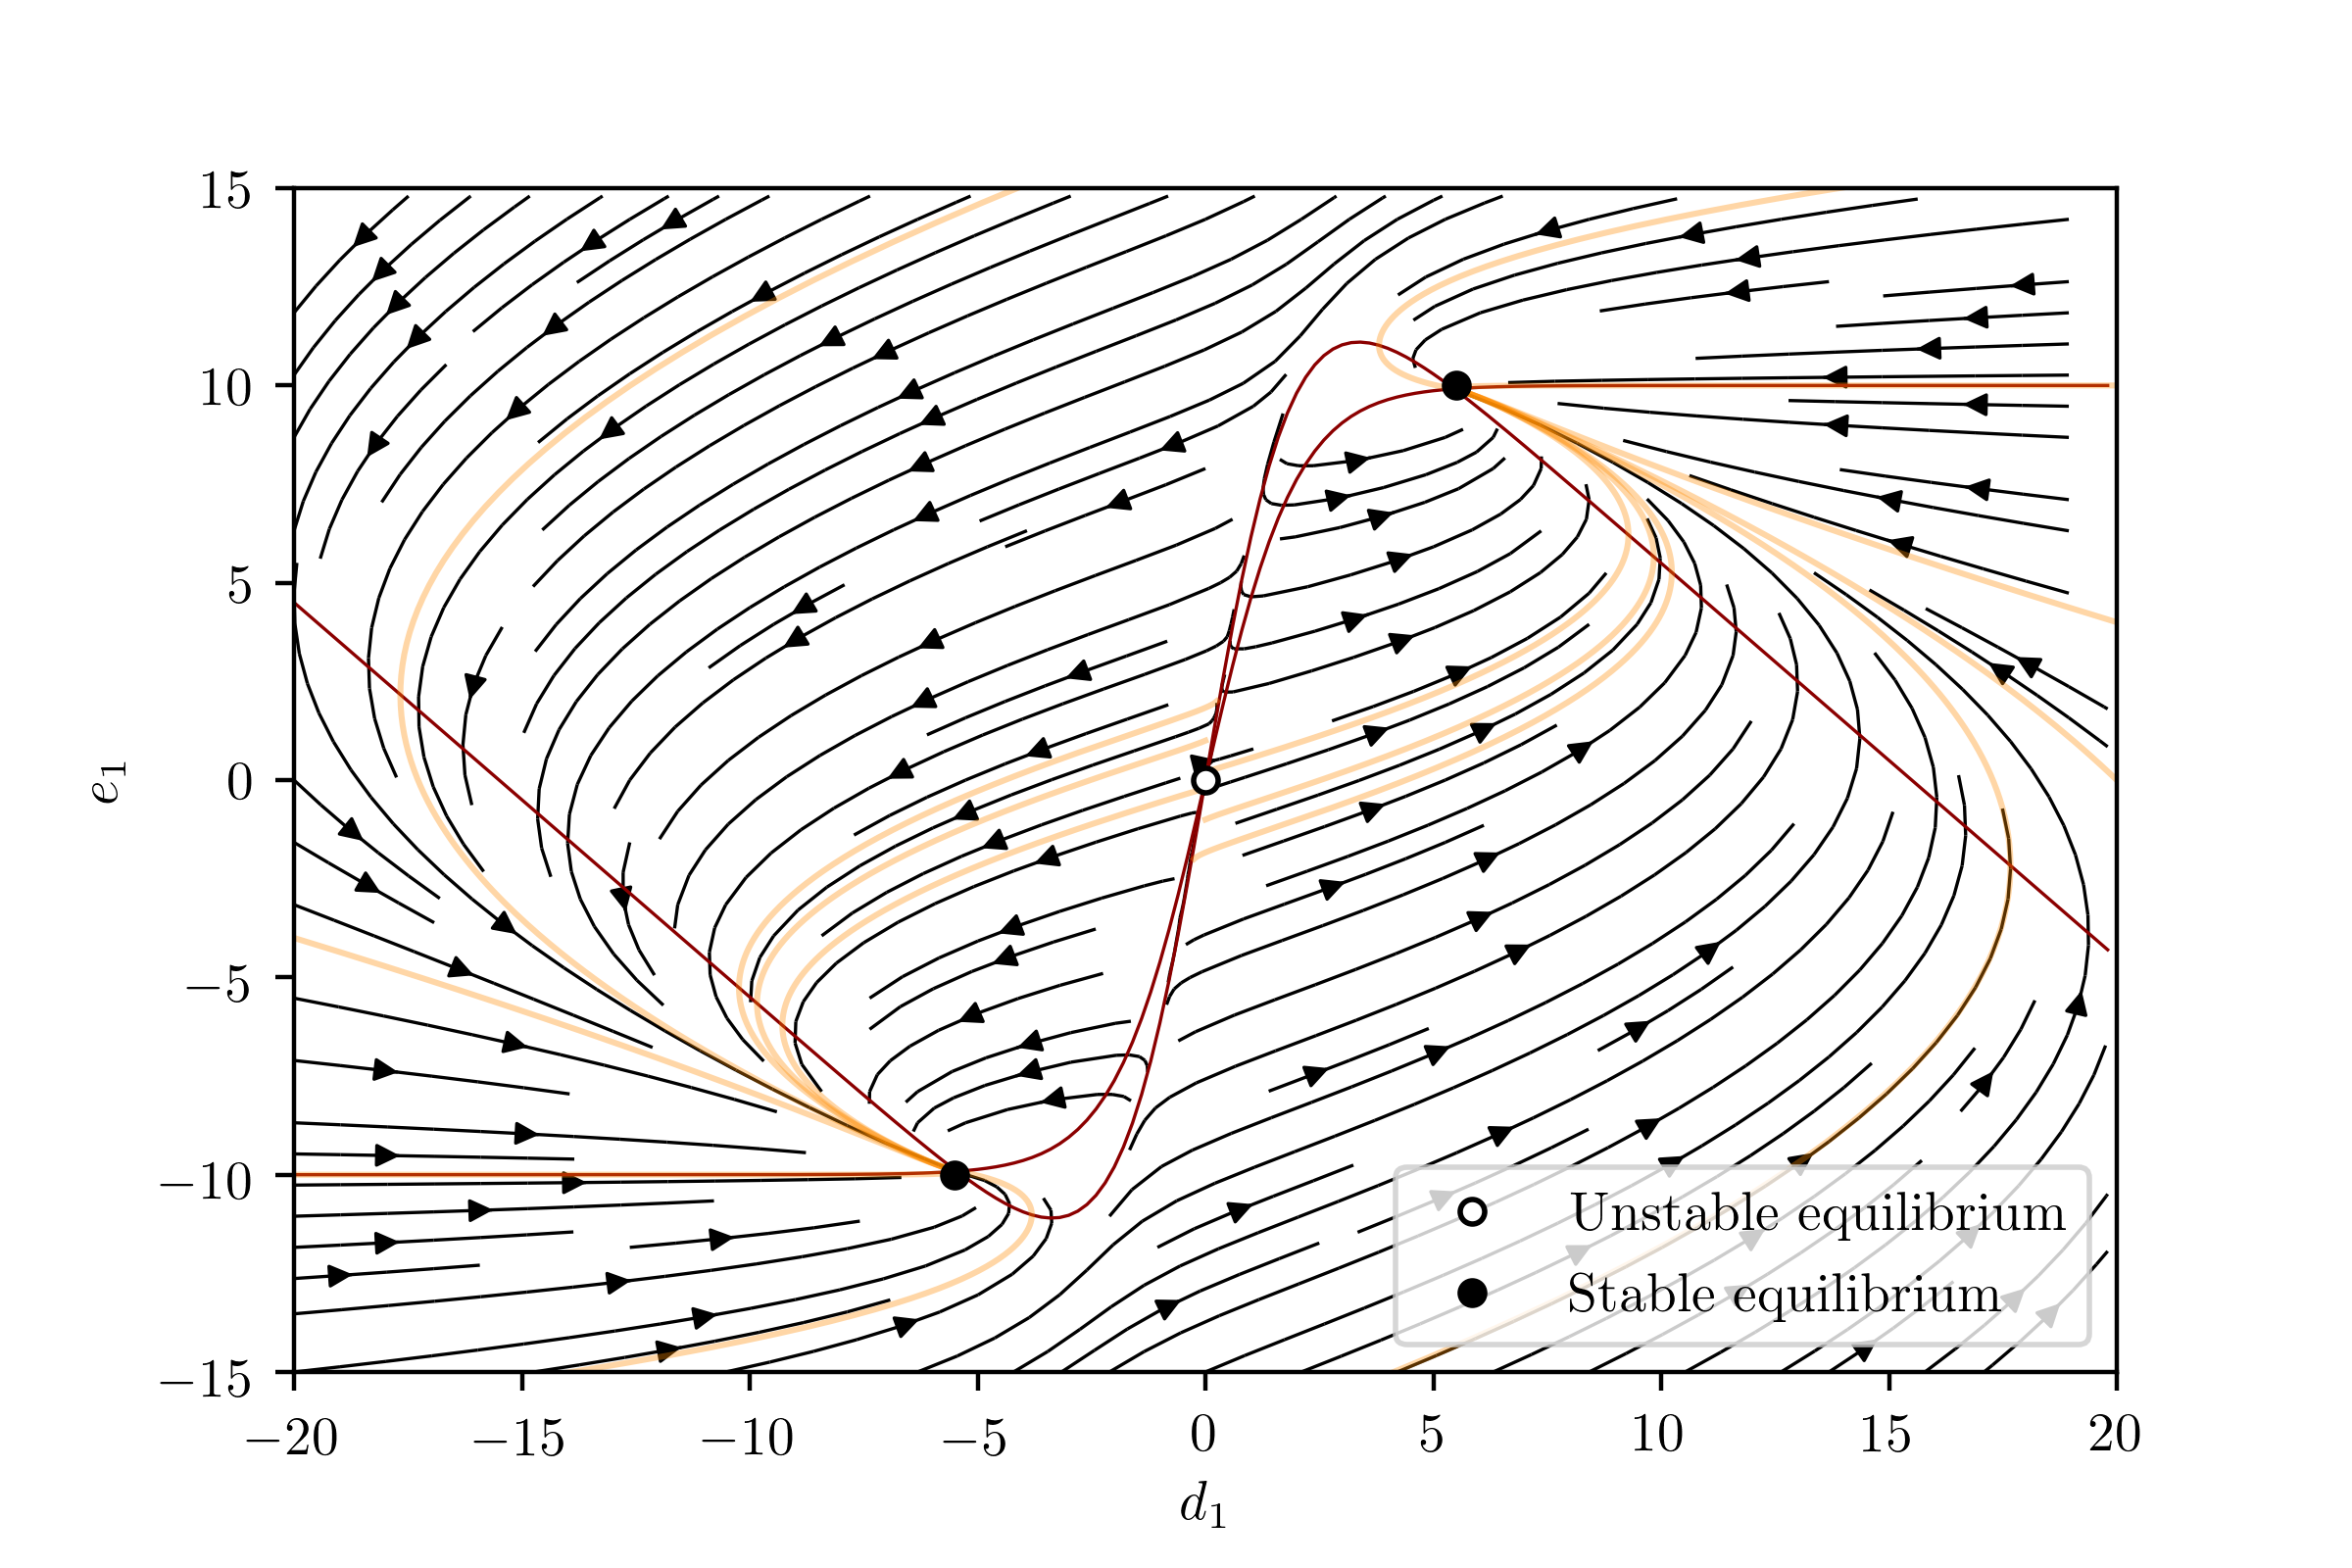
\includegraphics[width=\textwidth]{text/analysis/fig/2by2adapt/streamline_fixed.png}}
        \caption{\label{fig:eq2D_mem}Two equilibria}
\end{figure}